\chapter{预备知识}\label{chap:preliminaries}
\section{引言}
在开始介绍本文工作之前,首先需要了解一些背景知识。本章首先介绍什么是生成式模型和判别式模型,然后给出生成对抗网络的详细介绍及其数学模型,最后介绍InfoGAN和CatGAN模型。

\section{生成式模型和判别式模型}\label{sec:gm-dm}
在介绍生成对抗网络之前,我们有必要了解两个概念:生成式模型(Generative Modeling, GM)和判别式模型(Discriminative Modeling,DM)。我们先用简单地一句话说明,接着再详细阐述它们区别。简而言之,生成式模型研究的是数据和标签之间的联合分布,而判别式模型研究的是标签关于数据的条件分布。

在一个基本的机器学习问题中,通常有输入$x \in \Set{X}$和输出$y \in \Set{Y}$两个部分。通俗的说,DM关注$x$和$y$的内在联系,即在给定$x$的条件下,$y$的分布应该满足什么样的性质;
而GM更关注于$(x, y)$的联合分布。模型训练完成之后,判别式模型将训练数据集的信息提取,模型本身拟合了训练样本中的经验条件分布$P(y|x)$,因此对于测试样本$x^{\star}$,判别式模型直接输出对应的条件概率$P(y^{\star} | x^{\star})$,给出分类结果。生成式模型则对训练集的联合分布$P(x,y)$进行建模,对于未见样本$x^{\star}$,选择使得$P(x^{\star}, y)$最大的$y$作为预测值。由贝叶斯公式知
\[
  \begin{split}
    y^{{\star}} &= \argmax_y P(y|x^{{\star}}) \\
       &= \argmax_y \frac{P(x^{\star}|y)P(y)}{P(x^{\star})} \\
       &= \argmax_y P(x^{\star}|y)P(y) \\
       &= \argmax_y P(x^{\star}, y).
  \end{split}
\]
因此,这等价于寻找使得$P(y|x^{\star})$最大的$y$作为预测值。

常见的生成式模型有:朴素贝叶斯(Naive Bayes)、高斯混合模型(Gaussian Mixture Model,GMM)、受限玻尔兹曼机(Restricted Boltzmann Machine,RBM);常见的判别式模型有:KNN(K-Nearest Neighbours)、逻辑回归(Logistic Regression)、感知机(Perceptrons)、决策树(Decision Tree)、条件随机场(Conditional Random Field)等。
在实际使用中,两者各有优劣。生成式模型可以建模联合分布,但联合分布本身难以估计,所以会需要较大地数据量和计算量。判别式模型具有更低地渐近误差,但其收敛到渐近误差的速度比生成式模型更慢;而生成时模型的渐近误差往往高于判别式模型\citep{ng2002discriminative},而且可以处理隐变量和半监督甚至无监督学习。


%一般来说,判别式模型比生成式模型更受欢迎,特别是在分类问题中,判别式模型直接建模$P(y|x)$进行分类,而生成式模型则先建模$P(x,y)$然后再计算$P(y|x)$进行分类。首先联合概率的估计本身比较困难,因此需要耗费更多的数据量和计算资源。


\section{生成对抗网络}
\subsection{基本思想}
\citet{goodfellow2014generative}在2014年提出生成对抗网络,该模型使用博弈理论中的minimax博弈机制来训练两个模块:生成器和判别器。
%其目标是学习一个生成器对应的分布$p_g$使得它和真实数据的分布$p_{\text{data}}$尽量接近。
其目标时通过交替更新生成器和判别器,通过二者的对抗使得生成器学习到真实的数据分布,即令生成器对应的分布$p_g$和真实数据的分布$p_{\text{data}}$尽量接近。
生成式模型不直接估计每个数据样本的概率,而是利用生成网络$G$将噪声变量$\bd{z} \sim p_z(\bd{z})$映射到虚假样本$G(\bd{z})$。在训练过程中,判别器的目标是将虚假样本和真实样本区分开,生成器的目标则是生成让判别器无法区分的虚假样本。训练过程可以类比为两个玩家博弈:判别器读取一个数据希望能够分判定其是否为真实样本,而生成器希望生成以假乱真的数据从而让判别器判定为真。整个过程大致如下:生成器将一个随机噪声映射到数据空间,形成一个虚假数据。判别器接受真实样本或虚假样本作为输入,并输出当前样本来自真实数据的概率。训练的目标是一方面让判别器能够区分真假,一方面使生成器能够以假乱真,这就形成了两方对抗,最终二者的能力越来越强,无法进一步提高自己的性能,博弈达到平衡点。
\begin{figure}[htbp]
  \centering
  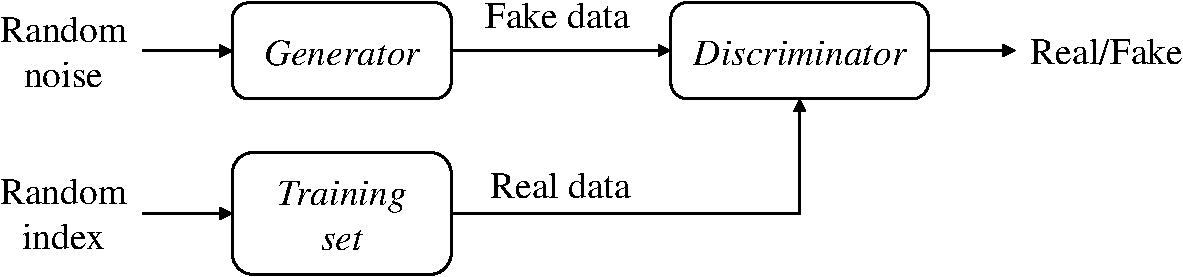
\includegraphics[width=0.9\textwidth]{Img/arch-gan.pdf}
  \bicaption{朴素GAN结构示意}{The architecture of vanilla GAN}
  \label{fig:arch-gan}
\end{figure}

\subsection{数学模型}
设$\Set{X} = \{\bd{x}_1, \cdots, \bd{x}_N\}$为含有$N$个样本的数据集,$\bd{x}_i = (x_{i1}, \cdots, x_{in}) \in \reals^n$为单个数据样本,标准生成对抗网络模型可被正式定义如下:生成器$G: \reals^m \mapsto \reals^n$,判别器$D: \reals^n \mapsto [0, ~1]$。其中$m$为隐空间维度,即噪声维度,$n$为数据维度。给定输入噪声$\bd{z} \sim p_z, \bd{z} = (z_1, \cdots, z_m) \in \reals^m$,$G(\bd{z}) \in \reals^n$为生成器生成的虚假样本;给定真实数据样本$\bd{x}$或虚假样本$G(\bd{z})$,$D(\cdot) \in [0,~1]$表示当前输入来自真实数据的概率。接着训练$D$使得对于真实数据$\bd{x}$,$D(\bd{x})$接近于$1$;对于虚假数据$\tilde{\bd{x}} = G(\bd{z})$,$D(\tilde{\bd{x}})$接近于$0$。同时训练$G$使得$\log(1 - D(G(\bd{z}))$达到最小。换言之,$D$和$G$类似两个玩家博弈,其价值函数如下:
\begin{equation}
  \min_G\max_D ~V(D,G) =
    \E_{\bd{x} \sim p_{\text{data}}}[\log D(\bd{x})] + 
    \E_{\bd{z} \sim p_z}[\log(1-D(G(\bd{z})))].
  \label{eq:gan-obj}
\end{equation}

在实际应用中,GAN通常被实现为可微神经网络:生成器网络$G(\cdot; {\theta}_g)$和判别器网络$D(\cdot; {\theta}_d)$,其中${\theta}_g$和${\theta}_d$分别为生成器和判别器的网络参数\footnote{为了简便起见,在不产生歧义的情况下通常省略网络参数。}。此外,生成器和判别器在实现中也需要采用交替迭代的机制,使用基于梯度的优化方法来训练。在训练初期,$G$生成的加虚假样本比较容易被$D$识别,从\eqref{eq:gan-obj}式可以看出,$\log(1 - D(G(\bd{z})))$的梯度变化很小,生成器难以得到优化。因此,在实现中通常训练$G$使得$\log D(G(\bd{z}))$达到最大。

%----------------------------------------------------------------------
\section{InfoGAN}\label{sec:infogan}
\subsection{基本思想}
朴素GAN通常使用高维高斯噪声作为生成器的输入,并没有规定生成器如何利用这个噪声,也没有对隐空间作任何限制。因此,噪声的利用可以是任意的,生成器可能生成具有高度耦合特征的数据。这从图像上来看,也就是模型生成的虚假图片高度抽象,没有明显轮廓。从底层来看,$\bd{z}$的每一维度并没有对应到生成数据的某个特征。然而,一个好的模型很自然地可以将数据的各个特征分离出来,以提供给用户调整。比如,当要求GAN从MNIST\citep{lecun1989backpropagation}生成图片时,理想的模型可以利用一个离散随机变量来表示数字类别特征(0-9),利用两个连续随机变量来分别表示数字的角度和笔画的粗细。

\citet{mirza2014conditional,odena2017conditional,miyato2018cgans}均指出通过调整隐空间结构,可以控制生成器生成具有某个特征的图片。InfoGAN\citep{chen2016infogan}将隐变量分解为两部分,一部分仍然是无结构的噪声$\bd{z} \sim p_z$,为模型提供足够的容量;另一部分则作为隐变量$\bd{c} \sim p_c$,用于学习数据特征。

\subsection{互信息约束}
设$\bd{c} = (c_1, c_2, \cdots, c_t)$表示输入空间中的$t$个隐变量,最简单的情况是各隐变量之间互相独立,即$p_{\bd{c}}(c_1, c_2, \cdots, c_t) = \prod_{i=1}^t p_{c_i}(c_i)$。InfoGAN基于朴素GAN模型提出了一种在无监督条件下,利用隐变量学习到数据特征的方法。该方法将隐空间噪声分解为两部分,包含一个生成器$G(\bd{z}, \bd{c})$和一个判别器$D$。由于在朴素GAN中,生成器可以忽略隐空间结构,此时$p_g(x|c) = p_g(x)$,其中$p_g$为生成器对应的概率分布。为了解决这个问题,InfoGAN为模型增加了互信息正则项,并指出隐变量$\bd{c}$和生成数据$G(\bd{z}, \bd{c})$之间的互信息应该很高。
\begin{figure}[hbtp]
  \centering
  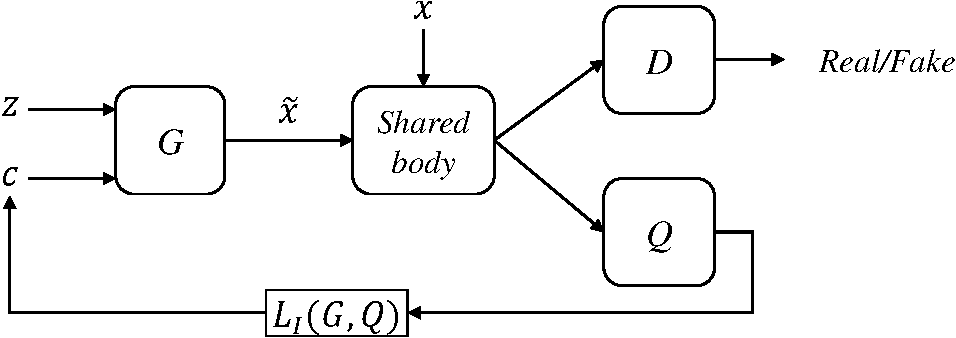
\includegraphics[width=0.75\textwidth]{Img/arch-infogan.pdf}
  \bicaption[InfoGAN结构示意]{InfoGAN结构示意。其中$\bd{x}$表示真实样本,$\tilde{\bd{x}} = G(\bd{z},\bd{c})$表示由生成器生成的虚假样本。在实现中,通常将辅助网络$Q$和判别器$D$共享一部分网络结构。}{The architecture of InfoGAN. $\bd{x}$ denotes the real data and $\tilde{\bd{x}} = G(\bd{z}, \bd{c})$ denotes fake data. In practice, $Q$ and $D$ share a body.}
  \label{fig:arch-infogan}
\end{figure}

在信息论中,熵(Entropy)、相对熵(Relative Entropy)以及互信息(Mutual Information)的定义如下\citep{cover2012elements}:
\begin{definition}{熵}
  设有离散随机变量$X \sim p_X(x)$及其支撑集$\Set{X}$,则它的熵$H(X)$定义为
  \begin{equation}
    H(X) = -\sum_{x\in\Set{X}} p_X(x) \log p_X(x).
  \end{equation}
  \label{def:entropy}
\end{definition}
\begin{definition}{KL距离}
  设有定义在同一个支撑集$\Set{X}$上的两个概率分布$p(x)$和$q(x)$,则它们的相对熵(或称Kullback-Leibler距离)定义为
  \begin{equation}
    D_{\text{KL}}(p~||~q) = \sum_{x\in\Set{X}} p(x)\log \frac{p(x)}{q(x)}.
  \end{equation}
  \label{def:relative-entropy}
\end{definition}
\begin{definition}{互信息}
  设$X,~Y$是两个离散随机变量,它们的支撑集分别为$\Set{X},~\Set{Y}$,它们的联合分布为$p_{X,Y}(x, y)$,边缘分布分别为$p_X(x)$和$p_Y(y)$,则$X$和$Y$之间的互信息$I(X;~Y)$定义为它们联合分布和边缘分布乘积之间的相对熵:
  \begin{equation}
    \begin{split}
      I(X;~Y) &= \sum_{x\in\Set{X}}\sum_{y\in\Set{Y}} 
      p_{X,Y}(x,y) \log\frac{p_{X,Y}(x,y)}{p_X(x) \cdot p_Y(y)}  \\
            &= D_{\text{KL}}\left( p_{X,Y}(x,y)~||~p_X(x) p_Y(y) \right) \\
            &= \E_{p_{X,Y}} \left[ 
              \log\frac{p_{X,Y}}{p_X \cdot p_Y}
              \right].
    \end{split}
    \label{eq:mutual-information}
  \end{equation}
  \label{def:mutual-information}
\end{definition}

在信息论中,熵度量着随机变量的其不确定性,用来衡量它所持有的信息量。由以上定义,容易得到
\begin{equation}
  \begin{split}
    I(X;~Y) &= H(X) - H(X|Y) \\
    &= H(Y) - H(Y|X).
  \end{split}
\end{equation}
可知随机变量$X,~Y$的互信息度量着观测到$Y$之后,$X$的不确定性的减少量。从\eqref{eq:mutual-information}式可以看出,互信息越大表明两个随机变量之间的相关性越大,反之互信息为零则说明变量间相互独立。于是,最大化隐变量$\bd{c}$和生成器输出$\tilde{\bd{x}} = G(\bd{z}, \bd{c})$的互信息$I(\bd{c}; ~\tilde{\bd{x}}) = H(\bd{c}) - H(\bd{c}|\tilde{\bd{x}})$等价于最小化$H(\bd{c}|\tilde{\bd{x}})$,这里由于$\bd{c}$的分布在整个过程中是确定的,所以$H(\bd{c})$可以视为常数。换句话说,隐变量$\bd{c}$的信息量在生成过程中应该流向$\tilde{\bd{x}}$,即给定$\tilde{\bd{x}}$之后,$\bd{c}$的信息量应该很小。类似的互信息约束也可以应用到聚类中\citep{bridle1992unsupervised,barber2006kernelized,krause2010discriminative}。InfoGAN在朴素GAN的基础上增加了互信息约束,其价值函数$V_I(D,G)$如下:
\begin{equation}
  \min_G\max_D ~V_I(D,G) = V(D,G) - \lambda I(\bd{c};~G(\bd{z},\bd{c})).
\end{equation}


\subsection{互信息的变分下界及其估计}
在实际应用中,由于依赖后验信息$p_{\bd{c}|\tilde{\bd{x}}}(c|x)$,互信息$I(\bd{c};~G(\bd{z},\bd{c}))$难以直接计算。\citet{poole2019variational}提出互信息的变分下界
\begin{equation}
  \begin{split}
    I(\bd{c}; \tilde{\bd{x}}) 
    &= \E_{ p_{\bd{c},\tilde{\bd{x}}} } \left[ 
      \log \frac{ p_{\bd{c},\tilde{\bd{x}}}(c, x) } 
                { p_{\bd{c}}(c) p_{g}(x) }
              \right] 
      = \E_{ p_{\bd{c},\tilde{\bd{x}}} } \left[ 
      \log \frac{ p_{\bd{c}|\tilde{\bd{x}}}(c|x) }
                { p_{\bd{c}}(c) }
              \right] \\
      &= \E_{ p_{\bd{c}, \tilde{\bd{x}}} } \left[
      \log \frac{ Q(c|x) }
                { p_{\bd{c}}(c) } 
              \right]
    + \E_{p_g(x)} \left[ 
      D_{\text{KL}} \left( p_{\bd{c}|\tilde{\bd{x}}}(c|x) ~||~ Q(c|x)
                    \right)
                  \right] \\
    &\ge \E_{ p_{\bd{c},\tilde{\bd{x}}} } \left[
      \log Q(c|x) \right] + H(\bd{c}) 
      \triangleq L_I(Q(c|x)),
  \end{split}
  \label{eq:vlb}
\end{equation}
其中$p_{\bd{c}}$为隐变量分布,$p_g$为生成器对应的概率分布,$Q(c|x)$为InfoGAN模型的辅助网络用以估计真实后验概率$p_{\bd{c}|\tilde{\bd{x}}}(c|x)$,$L_I(Q(c|x))$即为互信息的变分下界。在训练过程中,隐变量的分布是固定的,所以$H(\bd{c})$可视为常量。事实上,下界$L_I$与生成器和辅助网络都有联系:
\[
  L_I(G,Q) = \E_{ p_{\bd{c},\tilde{\bd{x}}} } \left[
  \log Q(c|G(\bd{z},\bd{c})) \right] + H(\bd{c}).
\]
从\eqref{eq:vlb}式可以看出,随着辅助分布$Q$接近真实后验分布,即
\[
  \E_{p_g(x)}[D_{\text{KL}}(p_{\bd{c},\tilde{\bd{x}}}(\cdot|x) ~||~ Q(\cdot|x))] \to 0,
\]
变分下界越来越紧。综上所述,InfoGAN的目标函数如下:
\begin{equation}
  \min_{G,Q}\max_D ~V_{\text{InfoGAN}}(D,G,Q) = V(D,G) - \lambda L_I(G,Q),
  \label{eq:infogan-obj}
\end{equation}
其中$\lambda$为正则系数。




%----------------------------------------------------------------------
\section{CatGAN}\label{sec:catgan}
\ref{sec:gm-dm}节提到生成式模型适合用于半监督甚至无监督学习,CatGAN\citep{springenberg2015unsupervised}就是研究无监督和半监督分类的模型。

\subsection{基本思想}
朴素GAN模型的判别器的输出是一个概率,代表着当前输入来自真实数据的概率。如前所述,GAN的训练过程可以表述如下。设有真实数据集$\Set{X} = \{\bd{x}_1, \cdots, \bd{x}_N\}$,$\bd{x}_i \in \reals^n$, $N$为数据样本个数。生成器$G$将噪声$\bd{z}\in \reals^m$映射到数据空间,生成虚假样本$\tilde{\bd{x}} = G(\bd{z})$。判别器$D$输出样本$x$来自真实数据集$\Set{X}$的概率:$\Pr(y=1 | x) = \frac{1}{1 + e^{-D(x)}}$。\eqref{eq:gan-obj}式可以写为如下等价形式:
\begin{equation}
  \min_G\max_D ~\E_{\bd{x} \sim p_{\text{data}}} \left[ \log \Pr(y=1|\bd{x}) \right]
  + \E_{\bd{z} \sim p_z} \left[ \log\left( 1 - \Pr(y=1|G(\bd{z})) \right) \right],
\end{equation}
其中$p_{\text{data}}$和$p_z$分别表示数据分布和噪声分布。朴素GAN没有对噪声分布作任何限制,CatGAN令$p_z = \text{Unif}(0,1)$,即连续均匀分布。

基于以上陈述,CatGAN提出了一种新的生成对抗网络结构来作无监督和半监督学习。首先考虑无监督的设定,无监督条件下的结构是针对朴素GAN的推广。

\subsection{问题建模}\label{sec:catgan-ps}
如前所述,设$\Set{X} = \{\bd{x}_1, \cdots, \bd{x}_N\}$为$N$个无标注数据样本。考虑以无监督的方式,从数据$\Set{X}$学习一个判别器$D$,使得$D$将给定数据划分到事先确定好的$K$个类别之一。进一步地,我们要求$D(\bd{x})$给出$\bd{x}$属于每个类别的概率:$\sum_{k=1}^K \Pr(y=k|\bd{x}) = 1$。CatGAN的目标是训练这样一个概率分类器,使其在分配概率时满足某种要求。注意到真实的标签分布是未知的,无法直接最大化对数似然函数,所以CatGAN了设计一个鉴定分类器性能的度量方式。具体说来,如果对于给定样本$\bd{x}$,$D$输出的条件分布$p(y|\bd{x})$具有很高的确定性,而边缘分布$p(y)$对于所有$k \in \{1,2,\cdots,K\} \triangleq [K]$都接近某个先验分布$p_Y$。在整个推导过程中,CatGAN假设标签的先验分布$p_Y$为类别均匀分布,也就是说$\Set{X}$中每个类别的样本数量大致相等:$\forall k_1, ~k_2 \in [K], ~\Pr(y=k_1) = \Pr(y=k_2)$。

上述问题的建模可以自然联想到软聚类问题,所以理论上来说可以用概率聚类算法如:Regularized information maximization (RIM) \citep{krause2010discriminative},或者最小化相对熵\citep{grandvalet2005semi}。然而一旦数据集中存在一些虚假相关性,这些方法就容易生过拟合。第二个直观感觉是朴素GAN的结构无法直接用来解决这个问题,因为朴素GAN的判别器只能输出一个概率以判断真假,而不能判断输入到底来自哪个类别。原则上,我们希望一个分类器可以建模数据分布,同时学习到数据特征加以利用进行下一步操作,比如判别式聚类。然而,判别器并不一定只能区分真假(二分类),它也应该能够将输入分配到多个类别。

尽管可能存在一些问题,但是一个非常简单的做法是将朴素GAN结构扩展一下使得判别器可被用于多分类任务。一旦$D$的结构改变,那么朴素GAN模型的对抗机制则需要重新设计。CatGAN将博弈机制改变为:要求判别器将每个真实数据样本划分到$K$个类别中的一个,而对于虚假样本,保持一个较高的不确定性。这样可以让分类器更加鲁棒。类似地,要求生成器生成具体到某个类别的图片而不是仅仅生成和真实数据类似的图片。

\subsection{目标函数}
如前所述,CatGAN所定义的优化问题与朴素GAN的不同之处主要在于:CatGAN想要学习一个判别器,它能够为每个真实数据样本$\bd{x}$附加一个标签$y \in [K]$而非学习一个二分类的判别器。定义判别器$D(\bd{x})$为可微函数,它输出一个$K$维对数概率向量(logits):$D(\bd{x}) \in \reals^K$。样本$\bd{x}$属于每个类别的概率可以通过对判别器输出施加softmax变换获得:
\begin{equation}
  \Pr(y=k|\bd{x}) = \frac{e^{D_k(\bd{x})}}{\sum_{k=1}^K e^{D_k(\bd{x})}},
\end{equation}
其中$D_k(\bd{x})$表示$D(\bd{x})$的第$k$个分量。和朴素GAN一样,生成器$G(\bd{z})$定义为将噪声$\bd{z} \in \reals^m$映射到数据空间$\tilde{\bd{x}} \in \reals^n$的函数:
\begin{equation}
  \tilde{\bd{x}} = G(\bd{z}), \quad \bd{z} \sim p_z,
\end{equation}
其中$p_z$表示噪声分布。

\begin{figure}[hbtp]
  \centering
  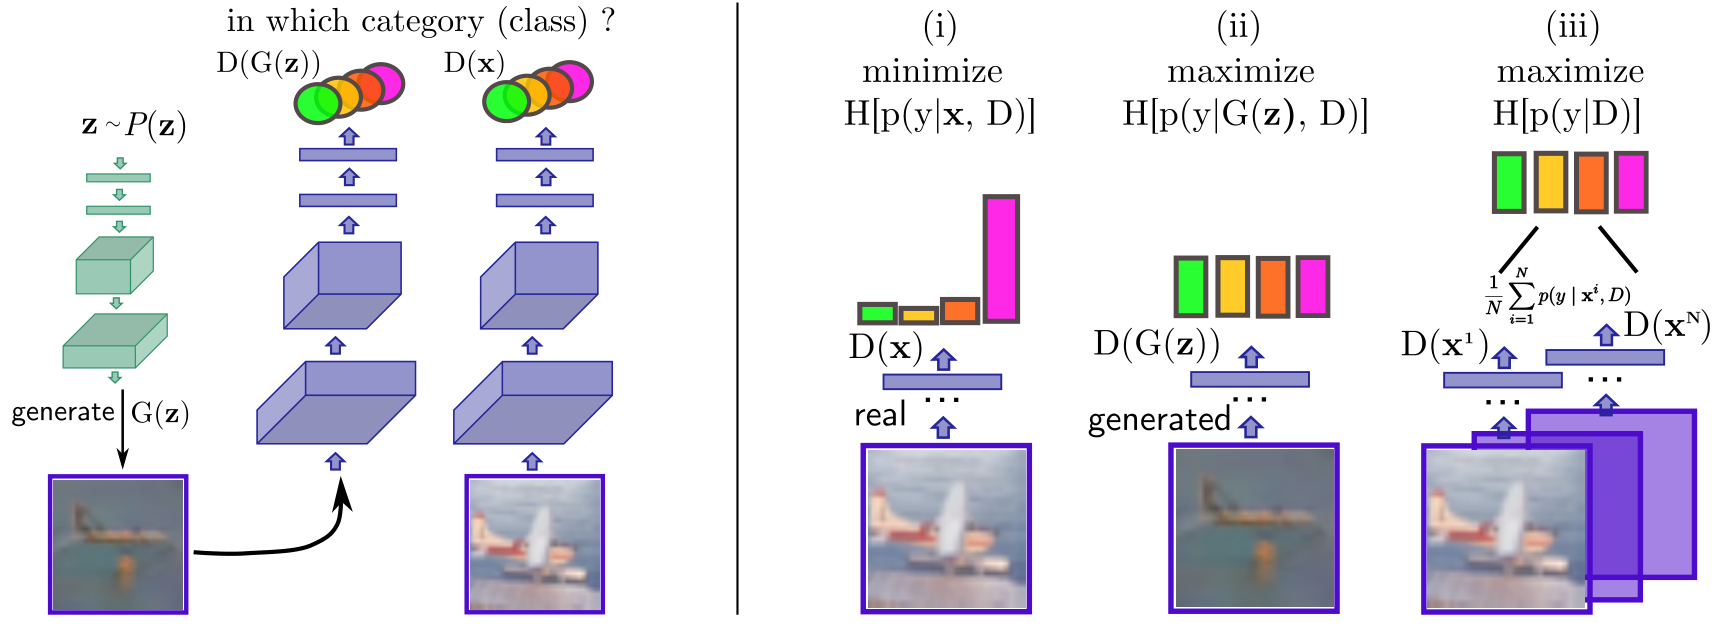
\includegraphics[width=0.9\textwidth]{Img/arch-catgan.png}
  \bicaption[CatGAN结构示意]
  {左图为CatGAN结构示意,绿色为生成器,紫色为判别器。右图为CatGAN判别器目标$L_D^{cat}$的直观解释。给定真实样本,判别器的输出呈单峰分布;给定虚假样本,判别器的输出呈均匀分布;对于所有真实图片,标签$y$的边缘分布呈均匀分布。}
  {The architecture of CatGAN is shown on the left, where generator is green and discriminator is violet. An intuitive interpretation of the objective function $L_D^{cat}$ for the discriminator is shown on right. For real samples, miminizing $H(p(y|\mathbf{x}))$ leads to single peak distribution; for fake samples, maximizing $H(p(y|G(\mathbf{z})))$ leads to uniform distribution. Finally, maximizing the marginal class entropy over all data-points leads to uniform usage of all classes.}
  \label{fig:arch-catgan}
\end{figure}

如\ref{sec:catgan-ps}节所说,如何度量分类器性能呢?CatGAN本意其实是让生成器作为判别器的正则项,使得判别器对于虚假样本更加鲁棒。基于这个想法,CatGAN提出了3条判别器需要满足的要求和2条生成器需要满足的要求:
\begin{itemize}
  \item[\textbf{判别器}](i) 对真实数据样本具有很高的确定性,(ii) 对于虚假样本具有很高的不确定性,(iii) 均匀使用所有类别\footnote{因为CatGAN假设标签的先验分布是类别均匀的。}。
  \item[\textbf{生成器}](i) 生成虚假样本使得判别器对其具有较高的确定性,(ii) 生成的样本均匀的分布在$K$个类别中。
\end{itemize}

CatGAN将这些要求都转化为可优化的条件概率,以此设计出目标函数。注意,在$K$个类别信息未知的情况下,我们无法直接优化条件概率$\Pr(y=k|\bd{x})$以满足判别器的第一个要求。因此,只能通过信息论中的一些尺度直接对分布信息进行刻画。最常用的信息论尺度就是熵。直观来看,对于真实样$\bd{x}$,我们想让条件分布$p(y|\bd{x})$呈现单峰趋势(即$D$很确定将当前样本划分到哪个类别),可以通过最小化$H(p(y|\bd{x}))$来满足判别器要求(i)。另一方面,对于虚假样本$\tilde{\bd{x}}$,我们想让条件分布$p(y|\tilde{\bd{x}})$呈现扁平化趋势(即$D$不确定将它划分到哪个类别),此时可以通过最大化$H(p(y|\tilde{\bd{x}}))$来满足判别器的要求(ii),当$H(p(y|\tilde{\bd{x}}))$达到最大时,$p(y|\tilde{\bd{x}})$在所有类别中均匀分布。因此,对于真实样本CatGAN定义其条件熵的估计
\begin{equation}
  \begin{split}
    \E_{ \bd{x} \sim p_{\text{data}} } \left[ H(p(y|\bd{x}) \right]
      &= \frac{1}{N} \sum_{i=1}^N H(p(y|\bd{x}_i)) \\
      &= -\frac{1}{N} \sum_{i=1}^N \sum_{k=1}^K \Pr(y=k|\bd{x}_i) \log\Pr(y=k|\bd{x}_i).
  \end{split}
  \label{eq:hy_given_x_real}
\end{equation}
对于虚假样本,条件熵的估计可以采用Monte-Carlo采样,使用$H(p(y|G(\bd{z})))$对噪声分布$p_z$取期望
\begin{equation}
  \E_{ \bd{z} \sim p_z } \left[ H(p(y|G(\bd{z}))) \right]
  \approx \frac{1}{M} \sum_{i=1}^M H(p(y|G(\bd{z}_i)))), \quad \bd{z}_i \sim p_z,
  \label{eq:hy_give_x_fake}
\end{equation}
其中$M$表示独立采样的噪声样本个数(CatGAN令$M=N$)。为了满足判别器和生成器的最后一个要求:均匀使用所有类别(对应均匀的边缘分布),CatGAN分别在真实数据集$\Set{X}$以及虚假样本集上定义边缘分布的熵估计:
\begin{equation}
  \begin{split}
    H_{\Set{X}}(p(y)) &= H\left( \frac{1}{N} \sum_{i=1}^N p(y|\bd{x}_i) \right), \\
    H_{G}(p(y)) &\approx H\left( \frac{1}{M} \sum_{i=1}^M p(y|G(\bd{z}_i)) \right), \quad \bd{z}_i \sim p_z.
  \end{split}
  \label{eq:hy}
\end{equation}
判别器和生成器分别最大化上面两个熵,其物理意义是对于判别器,希望均匀使用所有类别;对于生成器,希望生成的数据是类别均匀的。此时,判别器的要求(iii)和生成器的要求(ii)即可满足。对于生成器的要求(i),直接最小化\eqref{eq:hy_give_x_fake}式即可。注意,对于判别器,需要最大化\eqref{eq:hy_give_x_fake}式,其目的对虚假样本保持较高的不确定性;对于生成器,需要最小化\eqref{eq:hy_give_x_fake}式,其目的是希望判别器对于虚假样本具有较高的确定性,以判别为真。这样一来,就形成了对抗。CatGAN模型结构见图~\ref{fig:arch-catgan},图中给出了CatGAN目标函数的形象解释\footnote{CatGAN模型结构图摘自\citet{springenberg2015unsupervised}。}。

结合\eqref{eq:hy_given_x_real}\eqref{eq:hy_give_x_fake}\eqref{eq:hy}式我们可以得到CatGAN的目标函数$L_D^{cat}$和$L_G^{cat}$:
\begin{equation}
  \begin{split}
    L_D^{cat} &= \max_D ~H_{\Set{X}}(p(y)) 
    - \E_{\bd{x}\sim p_{\text{data}}} \left[ H(p(y|\bd{x})) \right]
    + \E_{\bd{z} \sim p_z}\left[ H(p(y|G(\bd{z}))) \right], \\
    L_G^{cat} &= \min_G ~-H_{G}(p(y)) 
    + \E_{\bd{z} \sim p_z}\left[ H(p(y|G(\bd{z}))) \right].
  \end{split}
  \label{eq:catgan-obj}
\end{equation}
以上给出的目标函数满足所有的设计要求,并且具有一定的可解释性:\eqref{eq:catgan-obj}式中$L_D^{cat}$的前两项可以合并为$I(p_{\text{data}};~p(y))$,其中$p(y)$预测标签分布。也就是说,判别器在最大化真实数据分布和预测标签分布之间的互信息,同时最小化虚假数据分布和预测标签分布之间的互信息。同理,对于$L_G^{cat}$前两项也可以合并为虚假样本和预测分布之间的互信息,这说明生成器想要最大化$I(p_g; ~p(y))$。很多判别式分类模型如感知机、逻辑回归等,都可以用信息论的角度解释为优化数据和标签之间的互信息,提取数据和标签相关的部分,寻找使得$\Pr(y|\theta(x)) = \Pr(y|x)$的充分统计量$\theta(x)$,作为模型所提取到的特征。这里,CatGAN也具有类似的可解释性。

\subsection{半监督学习}\label{sec:ss-catgan}
如果拥有少量标签信息,CatGAN就可以扩展到半监督学习模型,此时模型的性能可以达到进一步提升。考虑\ref{sec:catgan-ps}节所描述的问题,现在在原有的$N$个无标注数据样本上,额外增加$L$个带标签的数据$\Set{L} = \{\bd{x}_i, y_i\}_{i=1}^L$,使用$\bd{y}_i \in \reals^K$表示标签$y_i$经过one-hot编码之后的标签向量,即若$y_i = k$,则$\bd{y}_{ik} = 1$且对任意$j \neq k,~\bd{y}_{ij} = 0$。通过计算预测标签分布$p(y|\bd{x})$和$\Set{L}$上的真实标签分布之间的交叉熵,可以将这些有标签数据整合进\eqref{eq:catgan-obj}式中。给定一组$(\bd{x}, \bd{y})$,则预测标签分布和真实分布之间的交叉熵具有如下形式:
\begin{equation}
  \CE[\bd{y}, p(y|\bd{x})] = -\sum_{i=1}^K y_i \log\Pr(y=y_i|\bd{x}),
  \label{eq:cross-ent}
\end{equation}
其中$y_i$是标签向量$\bd{y}$的第$i$个分量。综上所述,可知半监督版本的CatGAN目标函数$L_D^{sscat}$和$L_G^{sscat}$具有如下形式:
\begin{equation}
  \begin{split}
    L_D^{sscat} &= L_D^{cat} + \lambda\E_{(\bd{x},\bd{y}) \in \Set{L}}
    \left[ \CE[\bd{y}, p(y|\bd{x})] \right], \\
    L_G^{sscat} &= L_G^{cat}, 
  \end{split}
  \label{eq:ss-catgan-obj}
\end{equation}
其中$\lambda$为正则化系数。

\section{本章小结}
本章介绍了生成对抗网络的基本思想及其数学模型。接着详细阐述了两种GAN的变体:InfoGAN和CatGAN。其中InfoGAN将噪声空间分解为无意义的噪声和有意义的隐变量,通过加入互信息正则项可以让隐变量学习到数据特征,并可以通过隐变量控制生成器的输出,为本文后续工作做了良好的铺垫。CatGAN则对朴素GAN中的判别器进行扩展,将原来的二分类扩展为多分类判别器,并利用判别器做无监督和半监督的多分类任务。


% \section{GAN 的研究展望}
% \subsection{克服模式坍塌}
% 模式坍塌是指 GAN 生成样本的模式总是集中
% 在少数几个甚至单一模式上,这导致数据生成结果
% 缺乏多样性[24]。因此,如何增加生成样本多样性是
% 亟待研究的内容:通过模型组合(如并行或级联)
% 对多个 GAN 的生成样本模式进行组合;利用推断
% 机制保证样本空间与隐变量空间的对应性,从而保
% 证生成器尽可能多地覆盖真实样本空间的所有模
% 式;将有效的多样性度量加入损失函数中,从而指
% 导模型训练等。
% \subsection{标准的评价指标}
% 对于生成模型这个研究领域来说,一个突出问
% 题是缺乏公认的定量评价指标,对于 GAN 来说也
% 是如此。生成样本的质量优劣仍依赖于主观判断,
% 而对于常用的客观评价指标,如平均对数似然,核
% 密度估计和生成样本的视觉保真度之间互不依赖
% 且分别适用于不同类型的生成模型,即使对相同类
% 型的生成模型,当应用对象不同时采用不同评估标
% 准也可能导致差别较大的训练效果。因此,如何对
% GAN 进行评估以及如何将 GAN 与其他类型的生成
% 模型进行比较是亟待解决的问题。
% \subsection{生成过程的可解释性}
% 早期研究工作着眼于模型的输出而忽视了模
% 型内部运作方式和产生输出的过程,解释 GAN 是
% 如何在无监督方式下“理解”图像和视频等数据的
% 研究工作至今鲜有报道。通过可视化手段解释模型
% 内部运作机理能更好地指导模型训练,如通过反卷
% 积操作将生成过程可视化,或激活某些中间层的特
% 征以表征和推断更高层次的特征。相信深度学习的
% 研究突破将为解决此问题提供新颖思路及技术手
% 段。\textcolor{magenta}{此外,通过增加从图像空间到隐变量空间的推
% 断过程,从而将隐变量的属性分离,也是使生成过
% 程可解释的有效手段。}
% \subsection{半监督学习}
% GAN 作为一种无监督学习方法被提出,可以对
% 无标签数据进行特征学习。尽管实际应用中难以获
% 得海量的标签数据,但获得少量标签数据往往是可
% 能的,实际应用结果表明,少量标签数据即能大大
% 提高 GAN 的表现。\textcolor{magenta}{因此,如何充分利用有限的标
% 签数据或对无标签数据自动添加标签,是 GAN 的
% 理论研究中具有广阔研究前景的方向之一。}
